

\fullcite{modm01}

%-------------------
\begin{multicols}{2}
\begin{center}
{\bf Article excerpts}
\\ 
{\bf Notes and remarks}
\end{center}
\end{multicols}


\begin{multicols}{2}
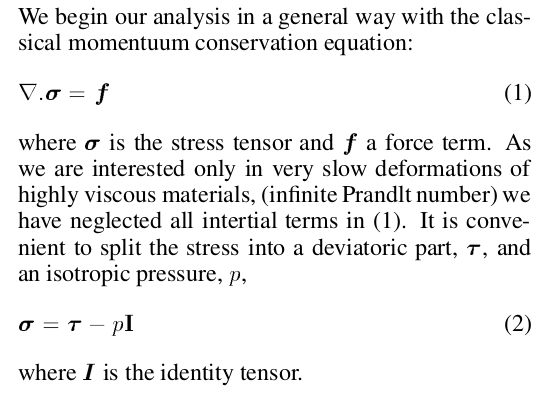
\includegraphics[width=8.25cm]{images/viscoelasticity/modm01a}\\
\[
\vec\nabla \cdot {\bm \sigma} + \vec{f} = \vec{0}
\]
\[
{\bm \sigma} = -p {\bm 1} + {\bm \tau}
\]
\end{multicols}

\begin{multicols}{2}
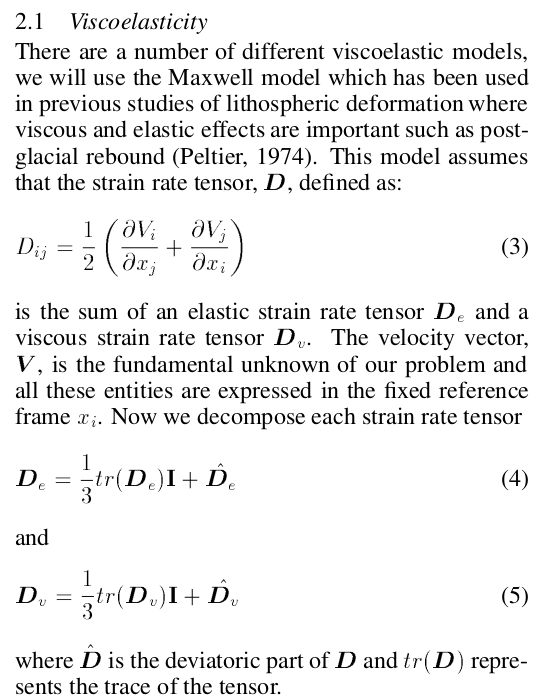
\includegraphics[width=8.25cm]{images/viscoelasticity/modm01b} \\
\[
\dot{\bm \varepsilon} = \frac12 (\vec\nabla \vec\upnu  + \vec\nabla \vec\upnu^T  ) 
\]

\[
\dot{\bm \varepsilon}_e = \frac13 {\rm tr}(\dot{\bm \varepsilon}_e) {\bm 1} + \dot{\bm \varepsilon}_e^d 
\]
\[
\dot{\bm \varepsilon}_v = \frac13 {\rm tr}(\dot{\bm \varepsilon}_v) {\bm 1} + \dot{\bm \varepsilon}_v^d 
\]
\end{multicols}

\begin{multicols}{2}
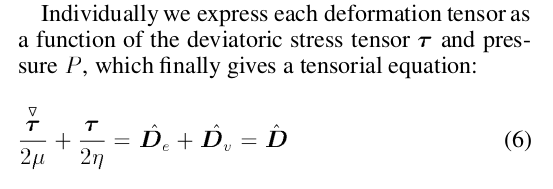
\includegraphics[width=8.25cm]{images/viscoelasticity/modm01c} \\
By taking the 'special' time derivative of the elastic equation we obtain  
\[
\frac{ \tilde{\bm \tau}}{2\mu} + \frac{{\bm \tau}}{2\eta}  
= \dot{\bm \varepsilon}_e^d + \dot{\bm \varepsilon}_v^d = \dot{\bm \varepsilon}^d 
\]
\end{multicols}

\newpage
\begin{multicols}{2}
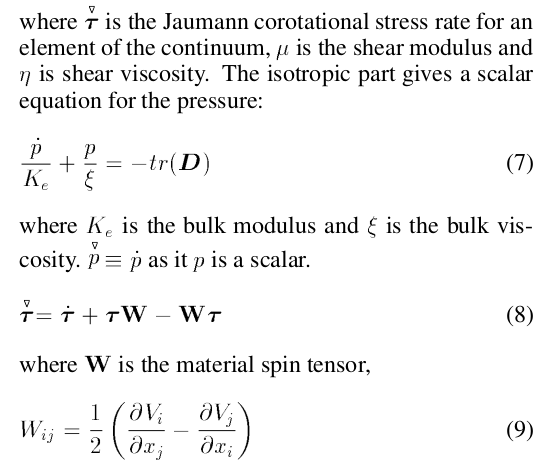
\includegraphics[width=8.25cm]{images/viscoelasticity/modm01d}\\
\[
\frac{\dot{p}}{K_e}+\frac{p}{\xi} = - {\rm tr} (\dot{\bm \varepsilon})
\]
\[
\tilde{\bm \tau} = \dot{\bm \tau} + {\bm \tau} \cdot \dot{\bm \omega} + \dot{\bm \omega} \cdot {\bm \tau}  
\]
\[
\dot{\bm \omega} = \frac12 (\vec\nabla \vec\upnu  - \vec\nabla \vec\upnu^T  ) 
\]

\end{multicols}

\begin{multicols}{2}
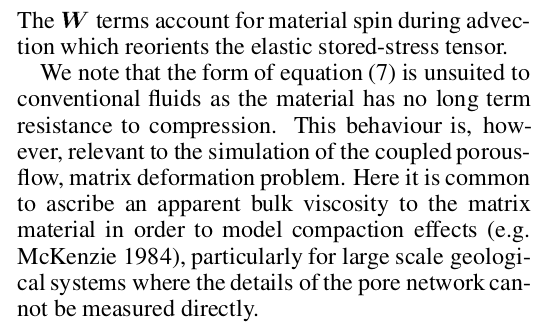
\includegraphics[width=8.25cm]{images/viscoelasticity/modm01e}\\
\end{multicols}

\begin{multicols}{2}
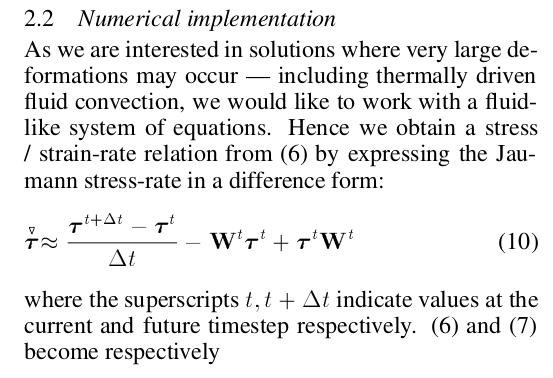
\includegraphics[width=8.25cm]{images/viscoelasticity/modm01f}\\
\[
\tilde{\bm \tau} = \frac{ {\bm \tau}^{t+\delta t} - {\bm \tau}^t }{\delta t} 
+ {\bm \tau}^t \cdot \dot{\bm \omega}^t + \dot{\bm \omega}^t \cdot {\bm \tau}^t  
\]

\end{multicols}

\begin{multicols}{2}
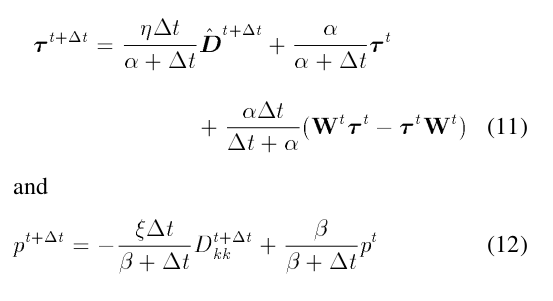
\includegraphics[width=8.25cm]{images/viscoelasticity/modm01g}\\
{\color{red} derive!!}
\[
{\bm \tau}^{t+\delta t} = \frac{\eta \delta t}{\eta/\mu + \delta t} {\bm \varepsilon}^{d,t+\delta t} + ...
\]
\[
p^{t + \delta t} = -\frac{\xi \delta t}{\xi/K_e + \delta_t } + \frac{}{} p^t
\]
\end{multicols}

\newpage
\begin{multicols}{2}
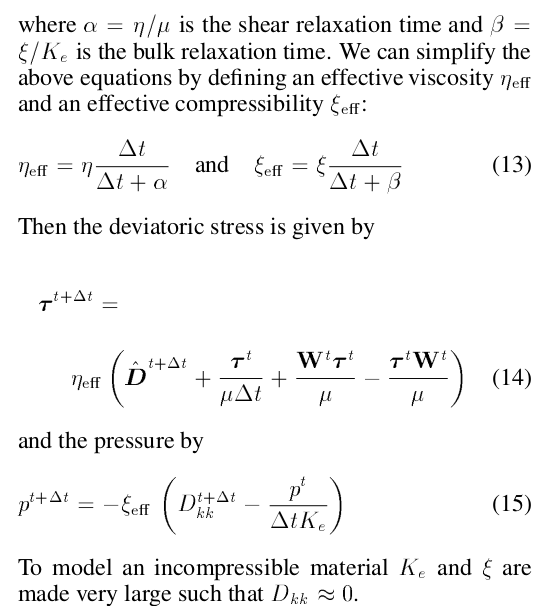
\includegraphics[width=8.25cm]{images/viscoelasticity/modm01h}\\
\end{multicols}

\begin{multicols}{2}
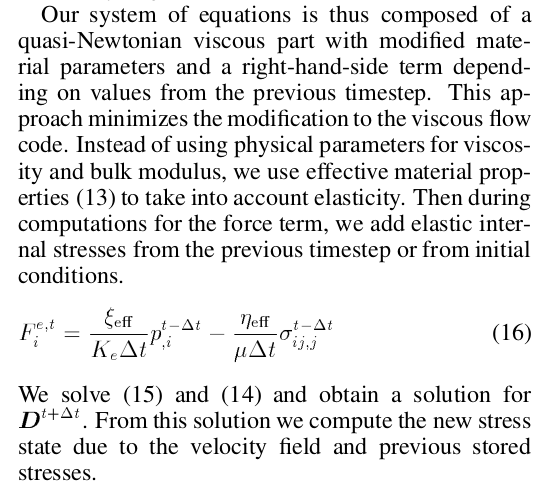
\includegraphics[width=8.25cm]{images/viscoelasticity/modm01i}\\
\end{multicols}

\begin{multicols}{2}
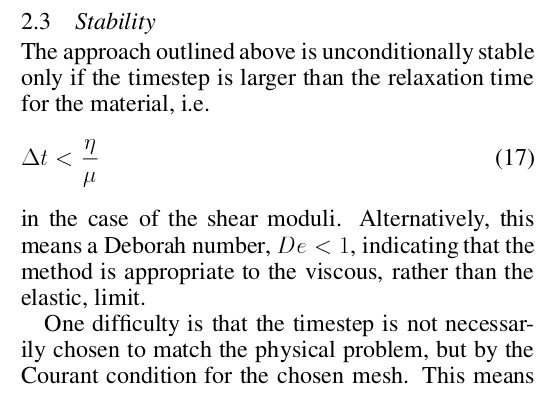
\includegraphics[width=8.25cm]{images/viscoelasticity/modm01j}\\
\end{multicols}

\begin{multicols}{2}
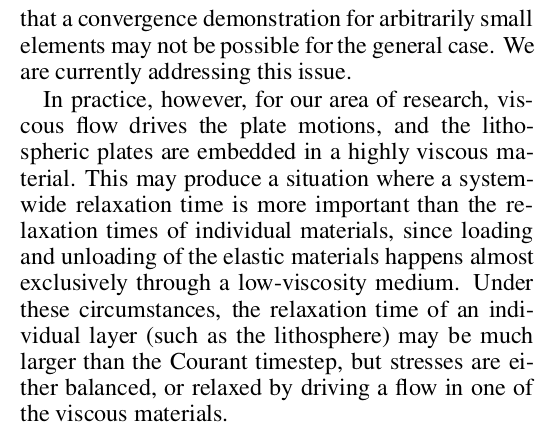
\includegraphics[width=8.25cm]{images/viscoelasticity/modm01k}\\
\end{multicols}

\begin{multicols}{2}
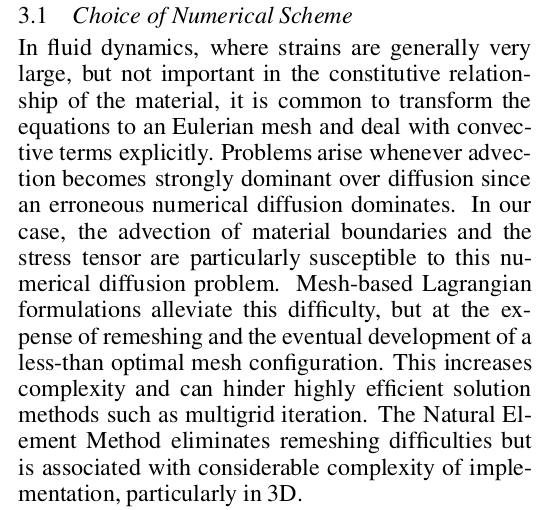
\includegraphics[width=8.25cm]{images/viscoelasticity/modm01l}\\
\end{multicols}

\begin{multicols}{2}
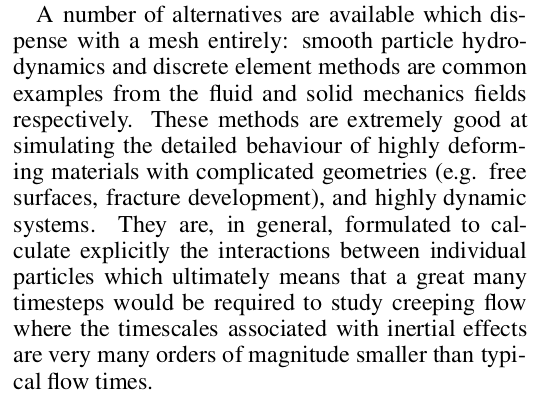
\includegraphics[width=8.25cm]{images/viscoelasticity/modm01m}\\
\end{multicols}

\newpage
\begin{multicols}{2}
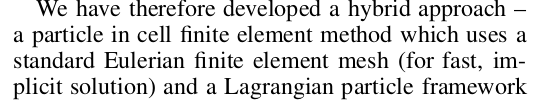
\includegraphics[width=8.25cm]{images/viscoelasticity/modm01n}
\end{multicols}

\begin{multicols}{2}
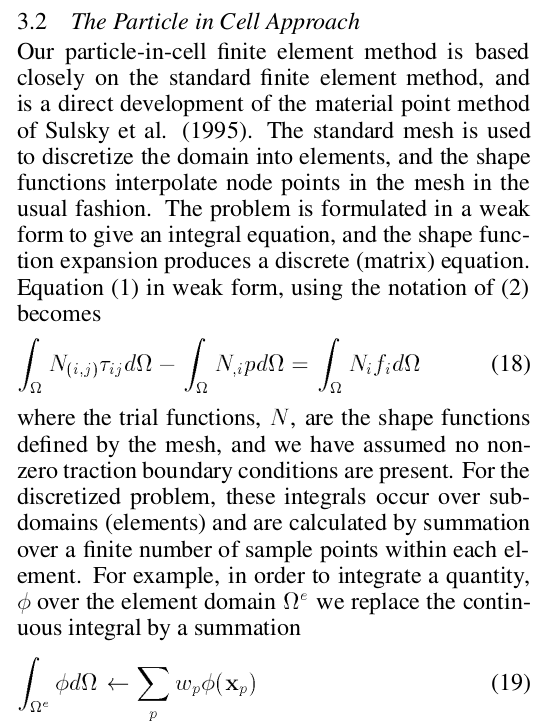
\includegraphics[width=8.25cm]{images/viscoelasticity/modm01p}\\
\end{multicols}

\begin{multicols}{2}
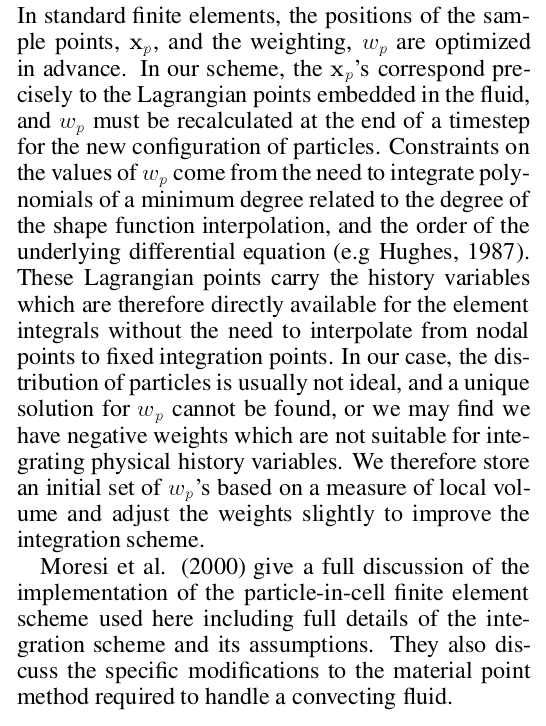
\includegraphics[width=8.25cm]{images/viscoelasticity/modm01q}\\
\end{multicols}



